\documentclass[11pt, oneside]{article}   	% use "amsart" instead of "article" for AMSLaTeX format
\usepackage[utf8]{inputenc}
\usepackage{geometry}                		% See geometry.pdf to learn the layout options. There are lots.
\geometry{letterpaper}                   		% ... or a4paper or a5paper or ... 
%\geometry{landscape}                		% Activate for rotated page geometry
%\usepackage[parfill]{parskip}    		% Activate to begin paragraphs with an empty line rather than an indent
\usepackage{graphicx}				% Use pdf, png, jpg, or eps§ with pdflatex; use eps in DVI mode
								% TeX will automatically convert eps --> pdf in pdflatex		
\usepackage{amssymb}
\usepackage{listings}
\usepackage{xcolor}
\usepackage[export]{adjustbox}
\usepackage{booktabs}
\usepackage{float}

\definecolor{codegreen}{rgb}{0,0.6,0}
\definecolor{codegray}{rgb}{0.5,0.5,0.5}
\definecolor{codepurple}{rgb}{0.58,0,0.82}
\definecolor{backcolour}{rgb}{0.95,0.95,0.92}

\lstdefinestyle{mystyle}{
	backgroundcolor=\color{backcolour},   
	commentstyle=\color{codegreen},
	keywordstyle=\color{magenta},
	numberstyle=\tiny\color{codegray},
	stringstyle=\color{codepurple},
	basicstyle=\ttfamily\footnotesize,
	breakatwhitespace=false,         
	breaklines=true,                 
	captionpos=b,                    
	keepspaces=true,                 
	numbers=left,                    
	numbersep=5pt,                  
	showspaces=false,                
	showstringspaces=false,
	showtabs=false,                  
	tabsize=2
}

\lstset{style=mystyle}

\title{Data Flow}
\author{Zelin Cai, Patrick Silvestre}
%\date{}							% Activate to display a given date or no date

\begin{document}
\maketitle

\section{\texttt{array\_merger.py}}
\begin{lstlisting}[language=Python]
__author__ = "Zelin Cai, Patrick Silvestre"
__version__ = "0.1.0"
__license__ = "MIT"

def array_merger(list1, list2):
	""" Variables to iterate through the lists """
	i = j = 0
	merged_list = []
	while i < len(list1) and j < len(list2):
		if list1[i] <= list2[j]:
			merged_list.append(list1[i])
			i += 1
		else:
			merged_list.append(list2[j])
			j += 1

	""" Checks if there are any index values remaining in list1 and appends them """
	while i < len(list1):
		merged_list.append(list1[i])
		i += 1

	""" Has the same purpose as the previous while loop but for list2 instead """
	while j < len(list2):
		merged_list.append(list2[j])
		j += 1

	return merged_list
\end{lstlisting}

\newpage
\section{\texttt{test\_array\_merger.py}}
\begin{lstlisting}[language=Python]
__author__ = "Zelin Cai, Patrick Silvestre"
__version__ = "0.1.0"
__license__ = "MIT"

from array_merger import *
import unittest


class TestTwoEmptyLists(unittest.TestCase):
	def test_01_two_empty_lists(self):
		"""
		Nodes:
		1-2-3-8-10-12
		"""
		list1 = []
		list2 = []
		expected_output = []
		actual_output = array_merger(list1, list2)
		self.assertEqual(expected_output, actual_output)


class TestOneEmptyList(unittest.TestCase):
	def test_02_first_list_empty(self):
		"""
		Nodes:
		1-2-3-8-
			10-11-
			10-12
		"""
		list1 = []
		list2 = [0]
		expected_output = [0]
		actual_output = array_merger(list1, list2)
		self.assertEqual(expected_output, actual_output)

	def test_03_second_list_empty(self):
		"""
		Nodes:
		1-2-3-
			8-9-
			8-10-12
		"""
		list1 = [0]
		list2 = []
		expected_output = [0]
		actual_output = array_merger(list1, list2)
		self.assertEqual(expected_output, actual_output)


class TestFullLists(unittest.TestCase):
	def test_04_list1_with_leftover_values(self):
		"""
		Nodes:
		1-2-
			3-4-6-7-
			3-4-6-7-
			3-4-6-7-
			3-
				8-9-
				8-9-
				8-9-
				8-9-
				8-10-12
		"""
		list1 = [3, 4, 5, 6]
		list2 = [0, 1, 2]
		expected_output = [0, 1, 2, 3, 4, 5, 6]
		actual_output = array_merger(list1, list2)
		self.assertEqual(expected_output, actual_output)

	def test_05_list2_with_leftover_values(self):
		"""
		Nodes:
		1-2-
			3-4-5-7-
			3-4-5-7-
			3-4-5-7-
			3-8-
				10-11-
				10-11-
				10-11-
				10-11-
				10-12
		"""
		list1 = [0, 1, 2]
		list2 = [3, 4, 5, 6]
		expected_output = array_merger(list1, list2)
		actual_output = array_merger(list1, list2)
		self.assertEqual(expected_output, actual_output)
\end{lstlisting}

\newpage
\begin{lstlisting}[language=Python]
	def test_06_same_sized_lists(self):
		"""
		Nodes:
		1-2-3-4-5-7-
			3-4-6-7-
			3-4-5-7-
			3-4-6-7-
			3-4-5-7-
			3-4-6-7-8-10-12
		"""
		list1 = [0, 2, 4]
		list2 = [1, 3, 5]
		expected_output = [0, 1, 2, 3, 4, 5]
		actual_output = array_merger(list1, list2)
		self.assertEqual(expected_output, actual_output)
\end{lstlisting}

\newpage
\section{Data Flow Graph}
\begin{figure}[!htb]
	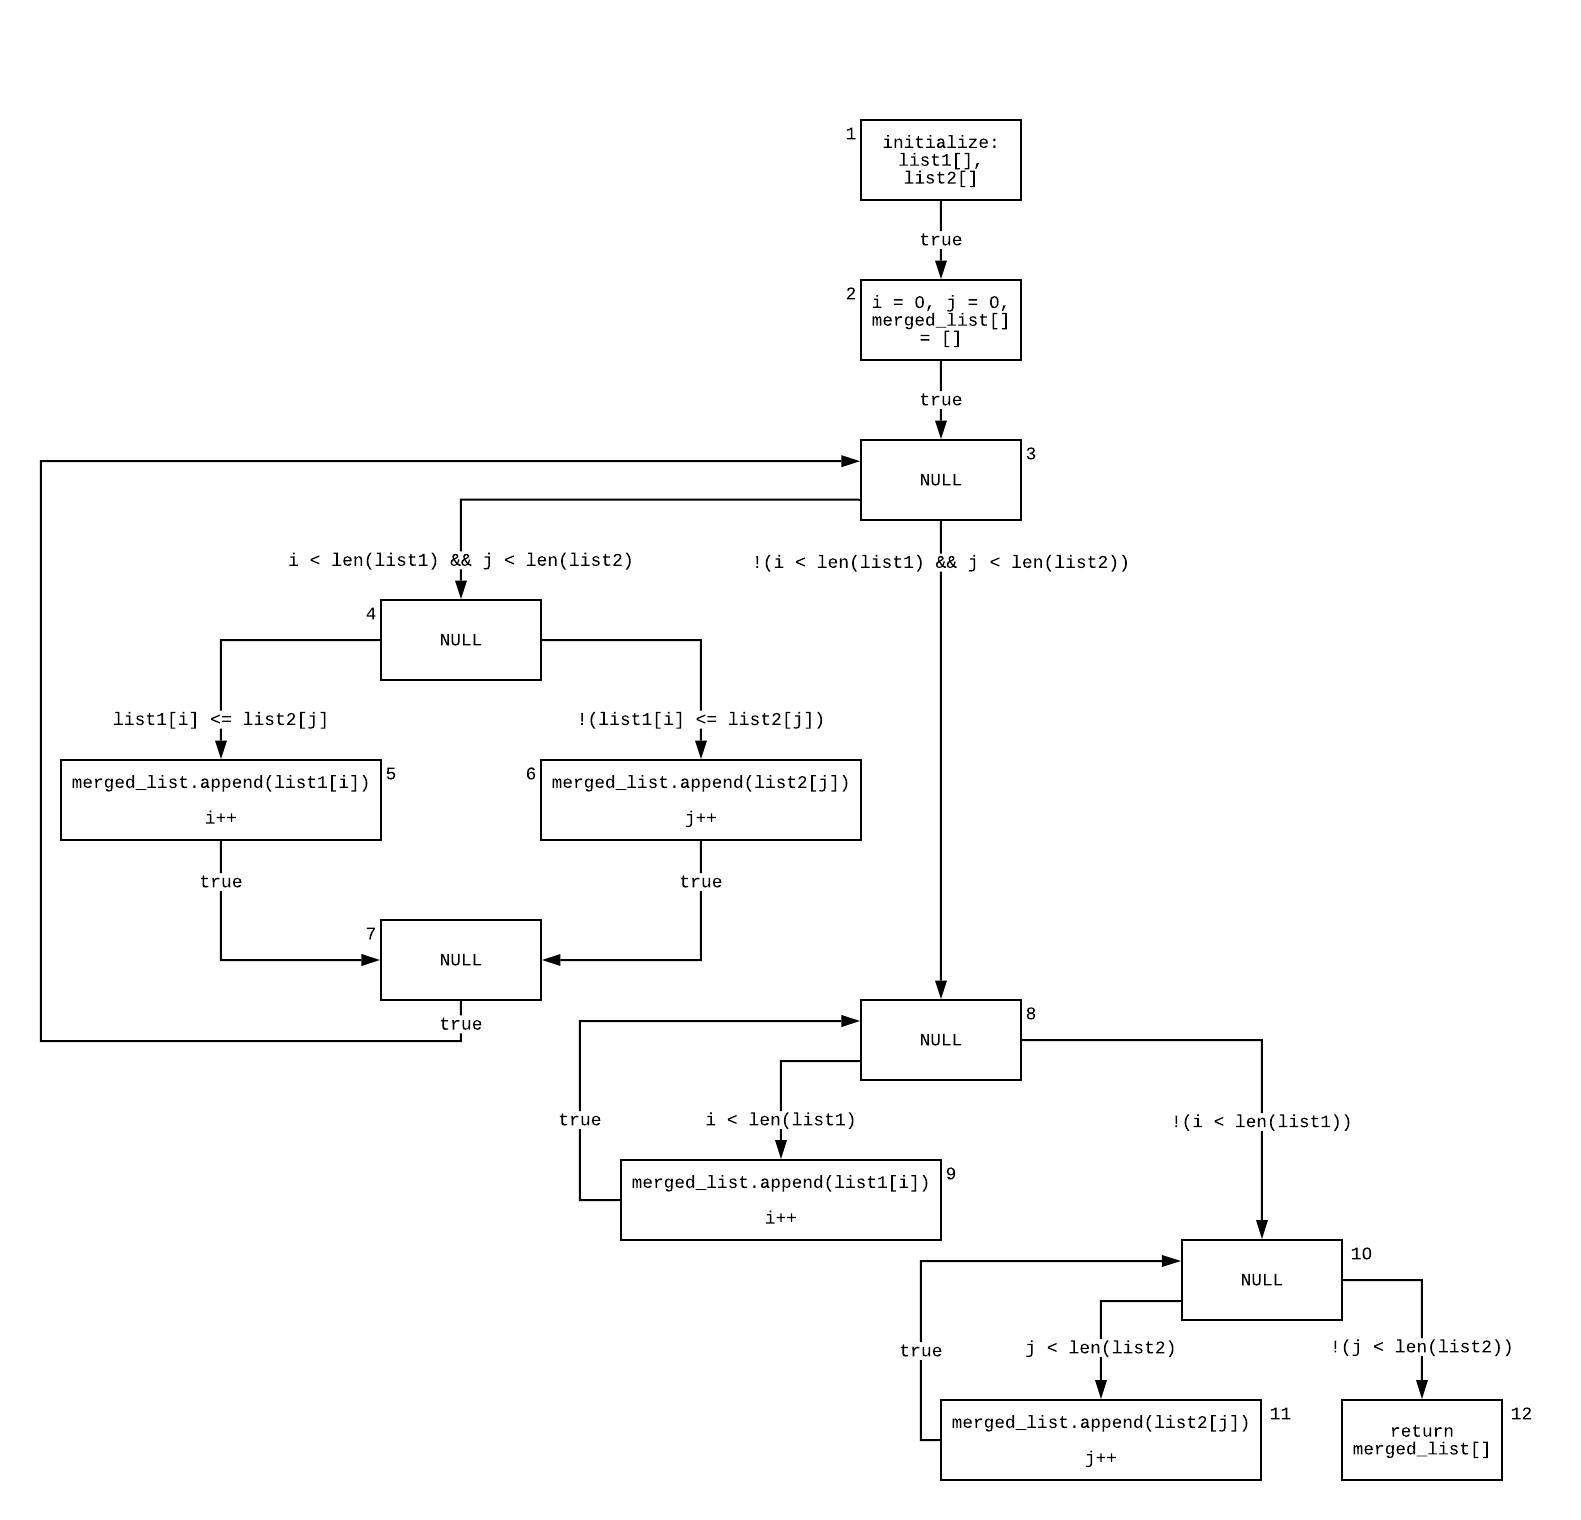
\includegraphics[max size={\textwidth}{\textheight}]{array-merger-data-flow-graph.png}
\end{figure}

\newpage
\section{Independent Paths}
\begin{enumerate}
	\item{1 - 2 - 3 - 8 - 10 - 12}
	\item{10 - 11 - 10}
	\item{8 - 9 - 8}
	\item{2 - 3 - 4 - 5 - 7}
	\item{3 - 4 - 6 - 7 - 3}
\end{enumerate}
\subsection{Simple Paths}
Paths 1, 2, 3, 4 and 5 are all simple paths since all of the nodes are distinct aside from the first and last nodes in paths 2, 3 and 5.
\subsection{Loop-Free Paths}
Paths 1 and 4 are loop-free paths since every node is distinct.

\newpage
\section{\texttt{def(), c-use(), p-use()}}
\begin{table}[H]
	\begin{tabular}{|l|l|l|}
		\hline
		Nodes \texttt{i} & \texttt{def(i)}                       & \texttt{c-use(i)}               \\ \hline
		1                & \{\texttt{list1{[}{]}, list2{[}{]}}\} & \{\}                            \\ \hline
		2                & \{\texttt{i, j, merged\_list{[}{]}}\} & \{\}                            \\ \hline
		3                & \{\}                                  & \{\}                            \\ \hline
		4                & \{\}                                  & \{\}                            \\ \hline
		5                & \{\texttt{merged\_list{[}{]}, i}\}    & \{\texttt{i, list1{[}i{]}}\}    \\ \hline
		6                & \{\texttt{merged\_list{[}{]}, j}\}    & \{\texttt{j, list2{[}j{]}}\}    \\ \hline
		7                & \{\}                                  & \{\}                            \\ \hline
		8                & \{\}                                  & \{\}                            \\ \hline
		9                & \{\texttt{merged\_list{[}{]}, i}\}    & \{\texttt{i, list1{[}i{]}}\}    \\ \hline
		10               & \{\}                                  & \{\}                            \\ \hline
		11               & \{\texttt{merged\_list{[}{]}, j}\}    & \{\texttt{j, list2{[}j{]}}\}    \\ \hline
		12               & \{\}                                  & \{\texttt{merged\_list{[}{]}}\} \\ \hline
	\end{tabular}
\end{table}

\begin{table}[H]
	\begin{tabular}{|l|l|l|}
		\hline
		Edges (i, j) & predicate(i, j)                                                  & p-use(i, j)                             \\ \hline
		(1, 2)       & \texttt{true}                                                    & \{\}                                    \\ \hline
		(2, 3)       & \texttt{true}                                                    & \{\}                                    \\ \hline
		(3, 4)       & \texttt{i \textless \ len(list1) \&\& j \textless\  len(list2)}  & \{\texttt{i, list1, j, list2}\}         \\ \hline
		(4, 5)       & \texttt{list1{[}i{]} \textless \ {}= list2{[}j{]} }              & \{\texttt{list1{[}i{]}, list2{[}j{]}\}} \\ \hline
		(4, 6)       & \texttt{!(list1{[}i{]} \textless{}= list2{[}j{]})}               & \{\texttt{list1{[}i{]}, list2{[}j{]}\}} \\ \hline
		(5, 7)       & \texttt{true}                                                    & \{\}                                    \\ \hline
		(6, 7)       & \texttt{true}                                                    & \{\}                                    \\ \hline
		(7, 3)       & \texttt{true}                                                    & \{\}                                    \\ \hline
		(3, 8)       & \texttt{!(i \textless \ len(list1) \&\& j \textless len(list2))} & \{\texttt{i, list1,j, list2\}}          \\ \hline
		(8, 9)       & \texttt{i \textless \ len(list1)}                                & \{\texttt{i, list1\}}                   \\ \hline
		(9, 8)       & \texttt{true}                                                    & \{\}                                    \\ \hline
		(8, 10)      & \texttt{!(i \textless \ len(list1))}                             & \{\texttt{i, list1\}}                   \\ \hline
		(10, 11)     & \texttt{j \textless \ len(list2)}                                & \{\texttt{j, list2\}}                   \\ \hline
		(11, 10)     & \texttt{true}                                                    & \{\}                                    \\ \hline
		(10, 12)     & \texttt{!(j \textless \ len(list2))}                             & \{\texttt{j, list2\}}                   \\ \hline
	\end{tabular}
\end{table}

\newpage
\section{Def-Use Associations and Associated Test Cases}
(When creating test cases, we attempted to follow the \emph{All du Paths Strategy}.)
\subsection{Variable \texttt{i}}
\begin{table}[H]
	\begin{tabular}{|l|l|l|}
		\hline
		du path                 & Test Case(s)     & (path)       \\ \hline
		(\texttt{i}, 2, (3, T)) & 4, 5, 6          & 2-3-4        \\ \hline
		(\texttt{i}, 2, (3, F)) & 1, 2, 3          & 2-3-8        \\ \hline
		(\texttt{i}, 2, (4, T)) & 5, 6             & 2-3-4-5      \\ \hline
		(\texttt{i}, 2, (4, F)) & 4, 6             & 2-3-4-6      \\ \hline
		(\texttt{i}, 2, 5)      & 5, 6             & 2-3-4-5      \\ \hline
		(\texttt{i}, 2, (8, T)) & 3, 4             & 2-3-...-8-9  \\ \hline
		(\texttt{i}, 2, (8, F)) & 1, 2, 3, 4, 5, 6 & 2-3-...-8-10 \\ \hline
		(\texttt{i}, 2, 9)      & 3, 4             & 2-3-...-8-9  \\ \hline
	\end{tabular}
\end{table}

\subsection{Variable \texttt{j}}
\begin{table}[H]
	\begin{tabular}{|l|l|l|}
		\hline
		du path                  & Test Case(s)     & (path)        \\ \hline
		(\texttt{j}, 2, (3, T))  & 4, 5, 6          & 2-3-4         \\ \hline
		(\texttt{j}, 2, (3, F))  & 1, 2, 3          & 2-3-8         \\ \hline
		(\texttt{j}, 2, (4, T))  & 5, 6             & 2-3-4-5       \\ \hline
		(\texttt{j}, 2, (4, F))  & 4, 6             & 2-3-4-6       \\ \hline
		(\texttt{j}, 2, 6)       & 4, 6             & 2-3-4-6       \\ \hline
		(\texttt{j}, 2, (10, T)) & 2, 5             & 2-3-...-10-11 \\ \hline
		(\texttt{j}, 2, (10, F)) & 1, 2, 3, 4, 5, 6 & 2-3-...-10-12 \\ \hline
		(\texttt{j}, 2, 11)      & 2, 5             & 2-3-...-11    \\ \hline
	\end{tabular}
\end{table}

\end{document}  